\documentclass[
BCOR 0.7cm,							% Bindekorrektur, bspw. 1 cm
11pt										% Schriftgroesse
]{scrbook}


\newif\ifpdf
\ifx\pdfoutput\undefined
	\pdffalse              	%normales LaTeX wird ausgef�hrt
\else
	\pdfoutput=1           
	\pdftrue               	%pdfLaTeX wird ausgef�hrt
\fi

\ifpdf
	%\usepackage{ae}        % Benutzen Sie nur
	%\usepackage{zefonts}  	% eines dieser Pakete
\else
	%%Normales LaTeX - keine speziellen Fontpackages notwendig
\fi

\ifpdf %%Einbindung von Grafiken mittels \includegraphics{datei}
	\usepackage[pdftex]{graphicx} %%Grafiken in pdfLaTeX
\else
	\usepackage[dvips]{graphicx} %%Grafiken und normales LaTeX
\fi


\ifpdf
	\pdfinfo
	{
    /Author (Manfred Kindl,Rudolf Hangl)                                
    /Title (WaWi)     
    /Subject (Benutzerhandbuch Warenwirtschaft)                                    
    /Keywords (WaWi Warenwirtschaft Technikum-Wien)
	}
\else			
\fi

\usepackage{listings} \lstset{numbers=left, numberstyle=\tiny, numbersep=5pt}
\lstset{language=tex} 


\usepackage[pdftex,colorlinks=true,urlcolor=blue,linkcolor=blue]{hyperref}
\usepackage[ngerman]{babel}		
\usepackage[T1]{fontenc}
\usepackage[left]{eurosym}
\usepackage[latin9]{inputenc}
\usepackage{makeidx}
\usepackage{float}
\usepackage[small,bf]{caption}
\usepackage{fancyhdr} %headerstyle
\usepackage{amssymb,amsmath}
\usepackage{color}


\addtokomafont{chapter}{\color[rgb]{0.0,0.376,0.584}}
\addtokomafont{section}{\color[rgb]{0.0,0.376,0.584}}
\addtokomafont{subsection}{\color[rgb]{0.0,0.376,0.584}}


\renewcommand{\rmdefault}{phv} % Arial
\renewcommand{\sfdefault}{phv} % Arial


\makeindex

\graphicspath{{../screenshots/}}

\setlength{\tolerance}{2000}
\setlength{\parindent}{0pt}
\setlength{\parskip}{1ex plus 0.5ex minus 0.2ex}
\addtolength{\textheight}{2cm}
\addtolength{\headheight}{2pt}
\setlength{\captionmargin}{20pt}
\floatstyle{plain}
\floatname{example}{Example}

\newfloat{example}{hbtp}{loe}[chapter]
\floatplacement{figure}{hbtp}
\floatplacement{table}{htbp}

\newcommand{\dollar}{\char36}
\renewcommand{\labelitemi}{
\includegraphics[width=5pt]{blacksquare}}
\renewcommand{\labelitemii}{--}
%\renewcommand*{\chapterformat}{\textcolor{red}}

\newenvironment{info}[1]{
    \hspace{-10mm}
    \fbox{
        \begin{minipage}{1cm}
        
\includegraphics[width=1cm]{icon_info}
        \end{minipage}
        \begin{minipage}{14.5cm}
        #1
        \end{minipage}
    }
}

\newenvironment{achtung}[1]{
    \hspace{-10mm}
    \fbox{
        \begin{minipage}{1cm}
        
\includegraphics[width=1cm]{icon_achtung}
        \end{minipage}
        \begin{minipage}{14.5cm}
        #1
        \end{minipage}
    }
}

\newenvironment{halt}[1]{
    \hspace{-10mm}
    \fbox{
        \begin{minipage}{1cm}
        
\includegraphics[width=1cm]{icon_halt}
        \end{minipage}
        \begin{minipage}{14.5cm}
        #1
        \end{minipage}
    }
}

\newenvironment{idee}[1]{
    \hspace{-10mm}
    \fbox{
        \begin{minipage}{1cm}
        
\includegraphics[width=1cm]{icon_idee}
        \end{minipage}
        \begin{minipage}{14.5cm}
        #1
        \end{minipage}
    }
}


\setlength{\unitlength}{1mm}

\newenvironment{markier}[5]{
    
    \thicklines \put(#2,#3){\vector(#4,#5){5}} \thinlines
    \put(#2,#3){\circle*{5}}
    \put(#2,#3){\textcolor{black}{\circle{5}}\makebox(-10,0){\textcolor{white}{#1}}}


}


\hyphenation{gleich-zeitig para-meter}


\begin{document}

\ifpdf
	\DeclareGraphicsExtensions{.pdf,.jpg,.png}
\else
	\DeclareGraphicsExtensions{.eps}
\fi

\pagestyle{fancyplain}

%% Titelseite einbinden %%%%%%%%%%%%%%%%%%%%%%%%%%%%%%%%%%%%%%%%%%%%%

%
% Titelseite, Abstrakt, Danksagung und Inhaltsverzeichnis
%
%% eigene Titelseitengestaltung %%%%%%%%%%%%%%%%%%%%%%%%%%%%%%%%%%%%%%%    

\begin{titlepage}
\begin{center}
\vspace*{40mm} \huge Benutzerhandbuch\\
\vspace*{10mm} 
%\huge WaWi\\
%\vspace*{10mm}
%\large \textsc{Warenwirtschaft}

\vfill 
\includegraphics[width=130mm]{wawi_logo_sz}
	
\large \vfill \textsc{FH Technikum Wien}\\

Wien, \today
\end{center}
\end{titlepage}

\tableofcontents			% Inhaltsverzeichnis
\frontmatter					% Vorspann (z.B. r�mische Seitenzahlen)
\chapter{Einleitung}
\info{Alle im Handbuch gezeigten Abbildungen wurden mit Daten aus der Entwicklungsdatenbank zur besseren Veranschaulichung der Abl�ufe erzeugt. Die Inhalte der Listen, wie etwa Betr�ge oder Zugriffsrechte, sind frei erfunden und haben keinen Bezug zu den Daten des Echtsystems.}
\mainmatter						% Hauptteil

%% Kapitel Anfang %%%%%%%%%%%%%%%%%%%%%%%%%%%%%%%%%%%%%%%%%%%%%%%%%

\setlength{\baselineskip}{0.5cm}
\chapter{Begriffserkl�rung}
\label{begriffe}

	\minisec{Konto}
Ein Konto dient der Darstellung von Gesch�fts- bzw. Verwaltungsvorf�llen.
Es verwaltet nur die reinen Ein- und Ausg�nge, also werden dort weder Gewinne noch Verluste ausgewiesen.

	\minisec{Kostenstelle}
Bezeichnet den Ort der Kostenentstehung und der Leistungserbringung. Sie wird nach Verantwortungsbereichen, r�umlichen, funktionalen, aufbauorganisatorischen oder verrechnungstechnischen Aspekten gebildet. Beispiele f�r funktionale Kostenstellen sind Materialkostenstellen, Fertigungskostenstellen, Forschungs- und Entwicklungskostenstellen, Verwaltungskostenstellen oder Vertriebskostenstellen.

	\minisec{Tag}
(['t{\ae}g], zu engl. �Etikett�)
Tag bezeichnet ein Schlagwort zur thematischen Einordnung eines Objekts. Ein Tag kann frei gew�hlt werden. Es dient dem leichteren Auffinden von Bestellungen bzw. der sinnvollen Zuordnung zu Themenbereichen. Es k�nnen sowohl einer ganzen Bestellung als auch einzelnen Posten innerhalb einer Bestellung Tags zugeordnet werden.\\
	Bei der Eingabe eines Tags, werden automatisch �bereinstimmungen mit vorhandenen Tags vorgeschlagen. W�hlen Sie entweder ein vorgeschlagenes Tag aus oder tippen Sie ein neues ein.
	Sie k�nnen auch mehrere Tags zuweisen. Trennen Sie diese mit einem Strichpunkt (;). Vermeiden Sie nach M�glichkeit Leer- und Sonderzeichen bei der Eingabe von Tags.
	
	\info{Wenn Sie bei einer Bestellung oder Bestellposition mehrere Tags definiert haben, werden diese auch bei der statistischen Auswertung mehrmals ber�cksichtigt und zur Gesamtsumme addiert. Zus�tzliche Tags verf�lschen also die Gesamtsumme.}
	
Verwendungsbeispiele:

\newcounter{fig}
\begin{list}{\textbf{Bsp. \arabic{fig}:}}{\usecounter{fig} \slshape}
\item Es wird B�romaterial bestellt. Als Tag definiere ich f�r die Gesamtbestellung den Begriff "`B�romaterial"'.
Bei den Berichten (siehe Kapitel \ref{bericht_tags}) wird nun die Summe aller Bestellungen, die als Tag "`B�romaterial"' definiert haben, aufgelistet.

\item In einer Bestellung bei der Firma XY wird ein Monitor und ein Textverarbeitungsprogramm bestellt.
Der Posten mit dem Monitor erh�lt den Tag "`Hardware"', der Posten mit dem Programm den Tag "`Software"'.
Bei den Berichten werden nun getrennt die Ausgaben f�r \textit{Hardware} und \textit{Software} erfasst.
\end{list}

\minisec{Bestellung}

Das Anlegen von Bestellungen dient in erster Linie der Vorausplanung und Vorab-Einteilung des Budgets.
Sie k�nnen das Bestellsystem auch nutzen, um sich einen �berblick �ber zuk�nftige Ausgaben zu verschaffen.
Solange die Bestellung nicht abgeschickt und freigegeben wurde, erfolgt auch keine tats�chliche Belastung des Budgets.

F�r einen besseren �berblick �ber die Ausgaben nutzen Sie besser die Rechnungssummen, da diese meist von der Bestellsumme abweichen (alte Katalogpreise, Skonti, Versandkosten,...).

Anschaffungen, die einen St�ckpreis von \EUR{250} �berschreiten, werden vom Inventarsystem erfasst.
Dabei werden die, bei den \textbf{Bestellungen} eingebenen Betr�ge ber�cksichtigt.
Wenn sich der tats�chliche Rechnungsbetrag vom Bestellbetrag unterscheidet, bessern Sie diesen bitte in der Bestellung aus,
um einen exakteren �berblick der vorhandenen Inventarwerte zu haben.

\minisec{Rechnung}

In den Rechnungen werden die tats�chlich gezahlten Betr�ge erfasst.
Bei den Berichten gibt Ihnen die Rechnungssumme also den genauen �berblick, wieviel vom Budget bisher tats�chlich belastet wurde.



\setlength{\baselineskip}{0.5cm}
\chapter{Benutzeroberfl�che}
\label{oberflaeche}
\begin{figure}
	\centering
	
\includegraphics[width=1\textwidth]{startfenster.png}
	\caption{Admin-Ansicht der Startseite (Sichtbare Bereiche je nach Berechtigung) }
	\label{oberflaeche}
\end{figure}

\section{Administrationsbereich \normalsize{(bei entsprechender Berechtigung)}}
\begin{description}
	\item [Konto:] (siehe Kapitel \ref{admin_konto}) �bersicht �ber alle vorhandenen Konten; bearbeiten und l�schen von Konten.
	\begin{description}
		\item [Neu:] Neues Konto anlegen.
		\item [Zusammenlegen:] Zum Zusammenfassen doppelt angelegter Konten.
	\end{description}
	\item [Kostenstelle:] (siehe Kapitel \ref{admin_kostenstelle}) �bersicht �ber alle vorhandenen Kostenstellen; bearbeiten und l�schen von Kostenstellen; Zuordnen von Konten zu Kostenstellen.
	\begin{description}
		\item [Neu:] Neue Kostenstelle anlegen.
		\item [Zusammenlegen:] Zum Zusammenfassen doppelt angelegter Kostenstellen.
  	\item [Budgeteingabe:] Zur Eingabe des Budgets pro Kostenstelle und Gesch�ftsjahr.
  \end{description}
\end{description}

\section{Benutzerbereich}
\begin{description}
 \item [Bestellung:](siehe Kapitel \ref{bestellung})
 \begin{description}
 	\item [Neu:] Zum Anlegen einer neuen Bestellung.
 	\item [Suchen:] Zum Suchen und anschlie�enden Bearbeiten einer vorhandenen Bestellung.
 \end{description}
 \item [Rechnung:](siehe Kapitel \ref{rechnung})
 \begin{description}
 	\item [Neu:] Zum Anlegen einer neuen Rechnung.
 	\item [Suchen:] Zum Suchen und anschlie�enden Bearbeiten einer vorhandenen Rechnung.
 \end{description}
 \item [Personensuche:] F�r die Suche nach Personen (Wie auf der CIS-Seite)
 \item [Firma:](siehe Kapitel \ref{firma})
 \begin{description}
 	\item [Neu:] Zur Neuanlage einer Firma.
 	\item [Suchen:] Zum Suchen einer bereits eingetragenen Firma.
 \end{description}
\end{description}

\section{Berichte}
\begin{description}
	\item [Kostenstelle:](siehe Kapitel \ref{bericht_kostenstelle}) �berblick �ber alle Kostenstellen mit Bestell- und Rechnungssumme und dem Restbudget.
	\item [Tags:](siehe Kapitel \ref{bericht_tags}) Auswertung und Berechnung abh�ngig von den zugeordneten Tags.
\end{description}
\setlength{\baselineskip}{0.5cm}
\chapter{Benutzerbereich}

\section{Bestellung}
\label{bestellung}

Der folgenden Abbildung k�nnen Sie den regul�ren Ablauf des Bestellvorgangs entnehmen.
\begin{figure}
	\centering
	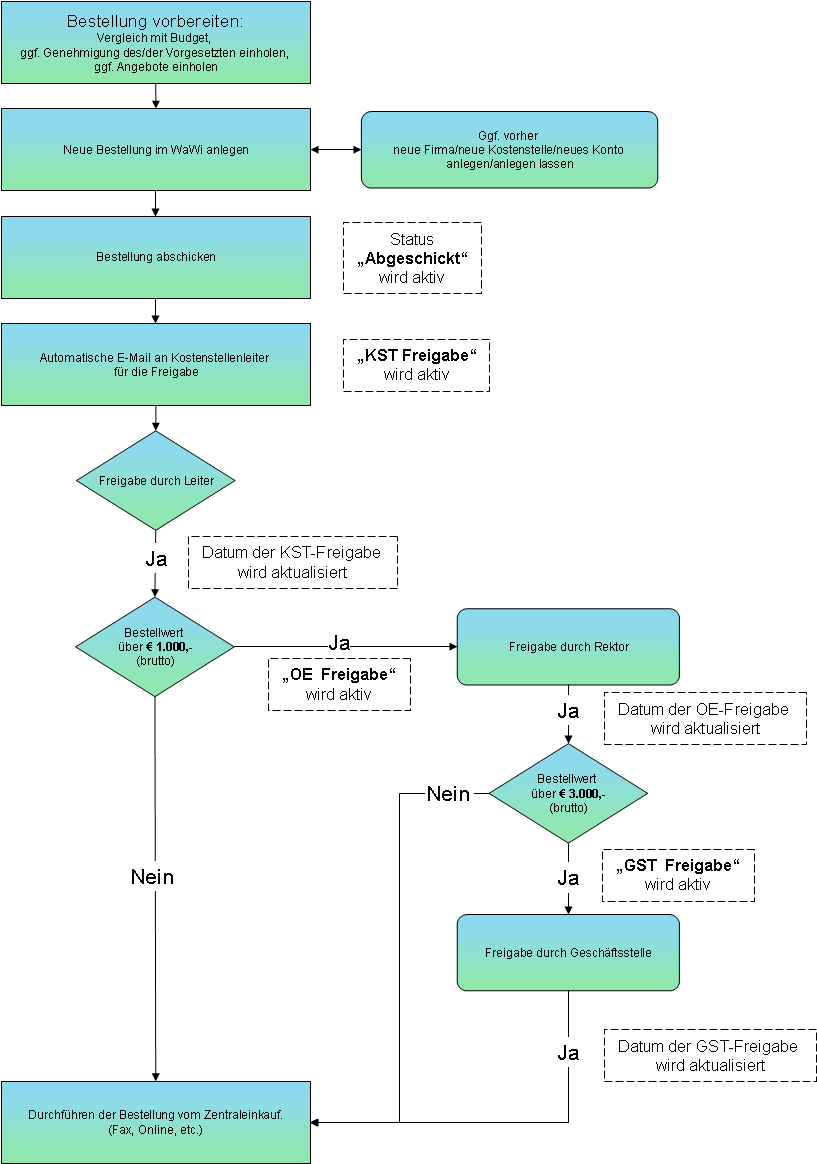
\includegraphics[width=0.8\textwidth]{workflow.png}
	\label{workflow}
\end{figure}

\subsection{Anlegen einer neuen Bestellung}
\label{neue_bestellung}

\begin{figure}
	\centering
	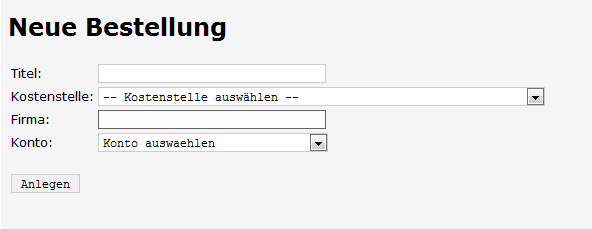
\includegraphics[width=0.8\textwidth]{neue_bestellung.png}
	\caption{Eingabeformular zum Anlegen einer neuen Bestellung }
	\label{neue_bestellung}
\end{figure}
Das Anlegen einer neuen Bestellung wird mit einem Klick auf den Men�punkt \textit{Neu} unter \textit{Bestellung} im linken Fenster begonnen. Es �ffnet sich danach die in Abbildung \ref{neue_bestellung} gezeigte Eingabemaske. \\
Hier sind vier Eingaben vorzunehmen:
\begin{description}
	\item [Titel:] Der Titel der Bestellung ist eine Kurzbeschreibung der Bestellung. Er vereinfacht das Wiederauffinden der Bestellung, da er als Suchkriterium verwendet werden kann. Der Titel erscheint auch auf dem Bestellformular.
	\item [Kostenstelle:] Auswahl jener Kostenstelle, die der Bestellung zugeordnet wird. Angezeigt werden nur Kostenstellen, f�r die der Nutzer/die Nutzerin Schreibrechte besitzt.
	\item [Firma:] Auswahl der Firma, bei der bestellt wird. Die Firma muss zuvor im WaWi angelegt worden sein. Die Auswahlliste der Firma wird nach Eingabe von mind. zwei Zeichen gefiltert. Unter der Firmenbezeichnung wird die ID der Firma in der Datenbank angezeigt.
	\item [Konto:] Auswahl, zu welchem buchhalterischen Konto die Bestellung zugeordnet wird. Die angezeigten Konten �ndern sich abh�ngig von der ausgew�hlten Kostenstelle.
\end{description}

\begin{figure}
	\centering
	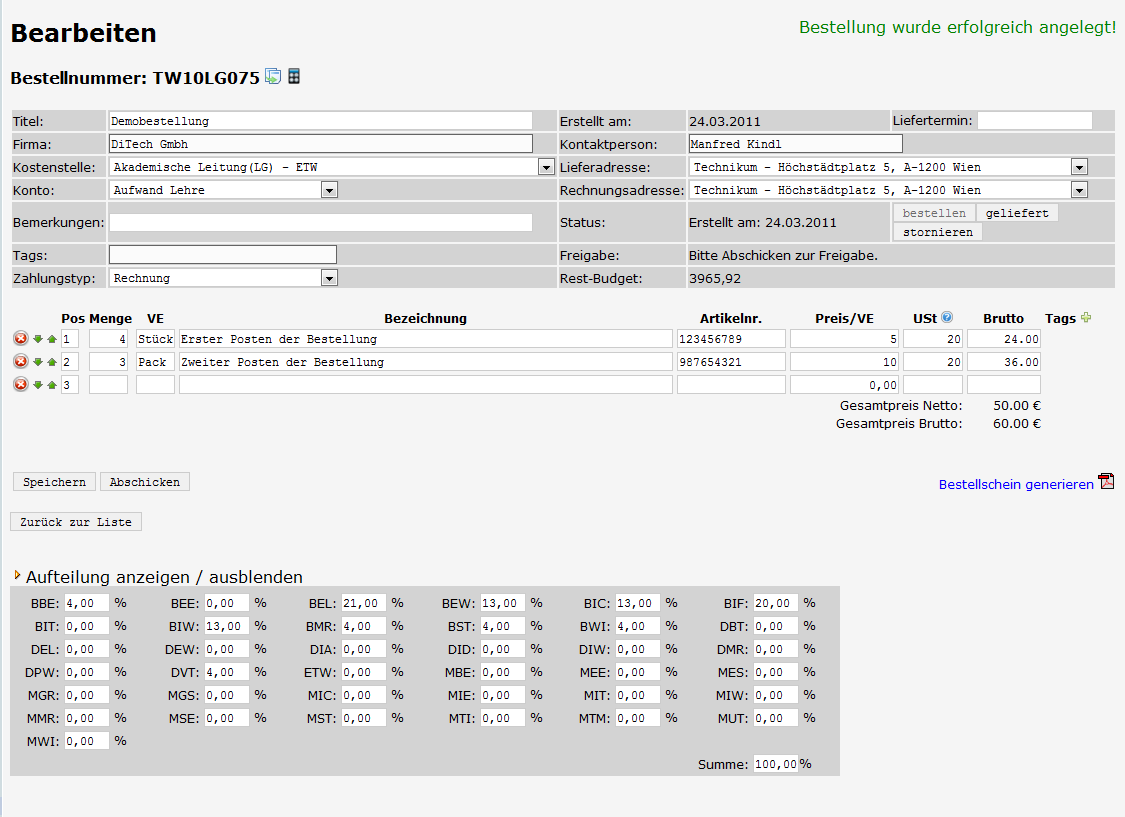
\includegraphics[width=1\textwidth]{bestellformular.png}
	\caption{Bestellformular}
	\label{bestellformular}
\end{figure}

\subsection{Angaben im Bestellformular}
\label{angaben_im_bestellformular}

Nach Klicken der Taste \textit{Anlegen} erscheint das eigentliche Bestellformular (siehe Abbildung \ref{bestellformular}):
\begin{description}
	\item [Bestellnummer:] Hier sehen Sie die automatisch generierte Bestellnummer. 
	Sie setzt sich zusammen aus der Organisationseinheit, dem Gesch�ftsjahr, dem K�rzel der Kostenstelle und einer fortlaufenden dreistelligen Nummer.
	Daneben finden Sie zwei Buttons. Der erste kopiert die Bestellung und �ffnet diese gleich zur Bearbeitung.
	Das Rechner-Symbol legt die zugeh�rige Rechnung an und �ffnet diese ebenfalls zur Bearbeitung.
\end{description}
	
	\info{Das nachtr�gliche �ndern der Bestellnummer ist nur m�glich, solange die Bestellung noch nicht bestellt wurde. Sollte sich danach die Kostenstelle �ndern,
	wird die Bestellnummer (das K�rzel der Kostenstelle) NICHT angepasst.}
	
\begin{description}
	\item [Titel:] Der Titel der Bestellung.
	\item [Erstellt am:] Das Erstellungsdatum der Bestellung.
	\item [Liefertermin:] Hier k�nnen Sie einen gew�nschten Liefertermin definieren, falls die Bestellung nicht promt stattfinden soll (zB: \textit{KW10} oder \textit{15.03.2011}).
	\item [Firma:] �ber den Firmennamen wird die Anschrift f�r das Bestellformular ausgew�hlt.
	\item [Kontaktperson:] Die Ansprechperson f�r die Bestellung.
	\item [Kostenstelle:] Die, der Bestellung zugeordnete, Kostenstelle.
	\item [Lieferadresse:] Die Adresse, an die die Bestellung geliefert werden soll.
	\item [Konto:] Buchhalterisches Konto.
	\item [Rechnungsadresse:] Die Empf�ngeradresse der Rechnung.
	\item [Bemerkungen:] Anmerkungen zur Bestellung k�nnen hier eingetragen werden. Bemerkungen werden NICHT auf dem Bestellschein gedruckt.
\end{description}
	\info{Bei Waren wie zB. techn. Einrichtungen, Laborger�ten, etc. bitte die Raumnummer dazu angeben. Dadurch erleichtern Sie uns die Erfassung im Inventarsystem}
\begin{description}
	\item [Status:] Zeigt den derzeitigen Bestellstatus an:
		\begin{itemize}
			\item Bestellen/Bestellt: Kann nur vom Zentraleinkauf aktiviert werden. Zeigt an, dass die Bestellung durchgef�hrt wurde (Fax, Onlinebestellung,...).
			\item Stornieren/Storniert: Wenn die Bestellung storniert wurde.
			\item Geliefert: Zeigt an, dass die Ware abholbereit ist bzw. geliefert wurde.
		\end{itemize}
	\item [Tags:] Ein Tag ist ein Schlagwort, welches frei gew�hlt werden kann. Es dient dem leichteren Auffinden von Bestellungen bzw. der sinnvollen Zuordnung zu Themenbereichen.
	Es k�nnen sowohl einer ganzen Bestellung als auch einzelnen Posten innerhalb einer Bestellung Tags zugeordnet werden.\\
	Bei der Eingabe eines Tags, werden automatisch �bereinstimmungen mit vorhandenen Tags vorgeschlagen. W�hlen Sie entweder ein vorgeschlagenes Tag aus oder tippen Sie ein neues ein.
	Sie k�nnen auch mehrere Tags zuweisen. Trennen Sie diese mit einem Strichpunkt (;). Vermeiden Sie nach M�glichkeit Leer- und Sonderzeichen bei der Eingabe von Tags.
	
	Beispiele f�r die Verwendung von Tags finden Sie in Kapitel \ref{begriffe}.
\end{description}

	\info{Wenn Sie bei einer Bestellung oder Bestellposition mehrere Tags definiert haben, werden diese auch bei der statistischen Auswertung mehrmals ber�cksichtigt und zur Gesamtsumme addiert. Zus�tzliche Tags verf�lschen also die Gesamtsumme.}
	
\begin{description}
	\item [Freigabe:] Hier wird nach dem Abschicken der Bestellung angezeigt, welche Abteilungen die Bestellung freigeben m�ssen (zB. Kostenstelle, Organisationseinheit).
	Wurde die entsprechende Freigabe erteilt, erscheint zus�tzlich das Datum der Freigabe neben der Abteilung.
	\item [Zahlungstyp:] Hier k�nnen Sie noch die Art der Zahlung �ndern. (Kreditkarte, Nachnahme, Rechnung, Vorauszahlung) 
		\begin{math}\rightarrow \end{math} Details siehe auch unter "`Workflows"' Kapitel \ref{workflows}.
\end{description}

	\info{Wenn Sie eine Bestellung per Nachnahme t�tigen, haben Sie daf�r zu sorgen, dass der entsprechende Betrag rechtzeitig beim Empfang hinterlegt ist}

\begin{description}
	\item [Rest-Budget:] Zeigt das verf�gbare Budget VOR dem Speichern der aktuellen Bestellung. Nach jedem Speichervorgang wird die Summe neu berechnet.
\end{description}

\subsection{Bestellpositionen innerhalb der Bestellung}

Jede Bestellposition wird in einer eigenen Zeile erfasst. Zu Beginn ist nur eine leere Zeile vorhanden.
Sobald Sie das Feld der Spalte \textit{Bezeichnung} verlassen, wird eine neue Zeile hinzugef�gt.
Folgende Eingabefelder stehen zur Verf�gung:
\begin{description}
	\item 
\includegraphics[height=3mm]{delete_round}: Dieser Button l�scht die jeweilige Zeile.
	\item 
\includegraphics[height=3mm]{arrow-single-down-green}: Schiebt diese Zeile um eine Zeile weiter nach unten.
	\item 
\includegraphics[height=3mm]{arrow-single-up-green}: Schiebt diese Zeile um eine Zeile weiter nach oben.
	\item [Pos:] Nummerierung des Postens. Standardm��ig erh�lt jede neue Zeile eine neue Postennummer.
	Wenn das nicht gew�nscht ist (weil zB. die neue Zeile nur Zusatztext aber keinen neuen Bestellposten enth�lt) kann die Nummerierung beliebig ver�ndert werden.
	\item [Menge:] Anzahl der zu bestellenden Ware.
	\item [VE:] Verpackungseinheit (St�ck, Pack, Meter, Rollen, usw.)( Max. 7 Zeichen).
	\item [Bezeichnung:] Beschreibung der Ware.
	\item [Artikelnr.:] Artikelnummer der Ware.
	\item [Preis/VE:] Nettopreis der Ware pro Verpackungseinheit. Der Bruttopreis wird automatisch nach Eingabe der USt berechnet.
	\item [USt:] Umsatzsteuer auf diese Ware. (Standardeinstellung 20\%). Durch einen Klick auf das Icon neben der USt �ffnet sich ein Fenster, dem Sie Details zur Eingabe der Umsatzsteuer entnehmen k�nnen. Die Internationale UID (Umsatzsteuer-Identifikationsnummer) wird links oben auf dem Bestellschein gedruckt.
	\item [Brutto:] Bruttopreis der Ware. Der Nettopreis wird automatisch nach Eingabe der USt berechnet.
	\item 
\includegraphics[height=3mm]{plus}: Damit blenden Sie die zus�tzliche Spalte \textit{Tags} ein.
	Sie k�nnen jeder Bestellposition Tags zuweisen. Zur Verwendung von Tags siehe unter \textit{Tags} im Kapitel \ref{angaben_im_bestellformular}.
\end{description}

\info{Wenn Sie einzelnen Posten innerhalb einer Bestellung Tags zuweisen, werden eventuell vorhandene Tags, die sich auf die Gesamtbestellung beziehen, ignoriert und bei den Berichten nicht ber�cksichtigt (siehe dazu auch Kapitel \ref{bericht_tags})}

\begin{description}
	\item [Speichern:] Diese Taste speichert die aktuellen Eingaben.
	\item [Abschicken:] Das Abschicken der Bestellung hat zur Folge, dass der Freigabe- und Bestellvorgang mit dem Versenden entsprechender Emails gestartet wird. 
	\end{description}
	
\achtung{Nach dem Abschicken k�nnen �nderungen in der Bestellung nur mehr von der Kostenstellenleitung durchgef�hrt werden}

\begin{description}
	\item [Erneut Abschicken:] (siehe Abbildung \ref{bestellformular_abgeschickt}) Nach dem erstmaligen abschicken der Bestellung wird dieser Button aktiv. Ein erneutes Abschicken versendet wiederholt eine E-Mail und kann verwendet werden um die Kostenstellenleitung an die Freigabe zu erinnern.
	\item [Statusinformation:] Hier sehen Sie, wann die Bestellung abgeschickt wurde.
	\item [Aufteilung anzeigen/ausblenden:] Hiermit wird die Aufteilung des Endbetrages auf die Studieng�nge angezeigt. Standardm��ig ist die Aufteilung ausgeblendet.
\end{description}

\begin{figure}
	\centering
	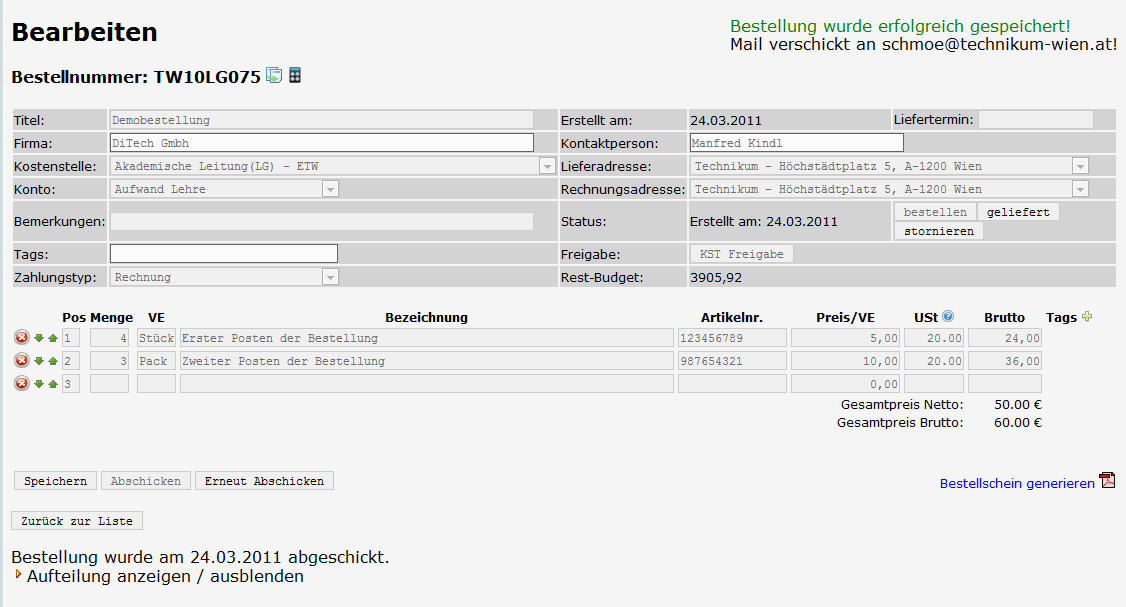
\includegraphics[width=1\textwidth]{bestellformular_abgeschickt.png}
	\caption{Bestellformular nach dem Abschicken}
	\label{bestellformular_abgeschickt}
\end{figure}

\subsection{Suchen nach einer Bestellung}
\label{suche_nach_bestellung}

Klicken Sie im Hauptmen� unter dem Punkt \textit{Bestellung} auf \textit{Suchen}. Hier k�nnen Sie nach vorhandenen Bestellungen suchen.

\begin{figure}
	\centering
	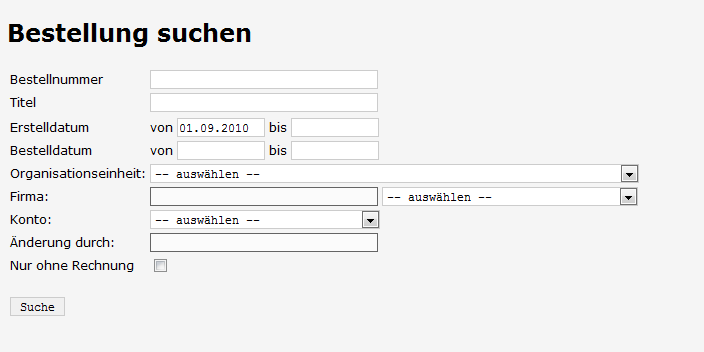
\includegraphics[width=1\textwidth]{bestellung_suchen.png}
	\caption{Bestellung suchen}
	\label{bestellung_suchen}
\end{figure}

Suchkriterien (alle optional):

\begin{description}
	\item [Bestellnummer:] Sucht nach der kompletten Bestellnummer oder Teilen davon.
	\item [Titel:] Sucht nach dem Titel einer Bestellung oder Teilen davon.
	\item [Erstelldatum/Bestelldatum:] Wenn Sie in das Feld klicken, erscheint ein Kalender, aus dem Sie das gew�nschte Beginn- und Enddatum w�hlen k�nnen.
	Sie k�nnen das Datum auch direkt in der Form TT.MM.JJJJ eingeben.
	\item [Organisationseinheit:] W�hlen Sie eine OE aus der Drop-Down Liste. Durchgestrichene OEs sind inaktiv.
	\item [Firma:] Auswahl der Firma, bei der bestellt wurde. Die Auswahlliste der Firma wird nach Eingabe von mind. zwei Zeichen gefiltert. Unter der Firmenbezeichnung wird die ID der Firma in der Datenbank angezeigt. Im Drop-Down Feld daneben werden die - zur OE zugeordneten - Firmen angezeigt, sofern welche vorhanden sind.
	\item [Konto:] W�hlen Sie hier das gew�nschte Verrechnungskonto aus.
	\item [�nderung durch:] Geben Sie hier den Namen der Person ein, die die Bestellung zuletzt ge�ndert hat.
	\item [Nur ohne Rechnung:] Es sollen nur Bestellungen aufgelistet werden, zu denen noch keine Rechnung eingetragen wurde.
\end{description}

\begin{figure}
	\centering
	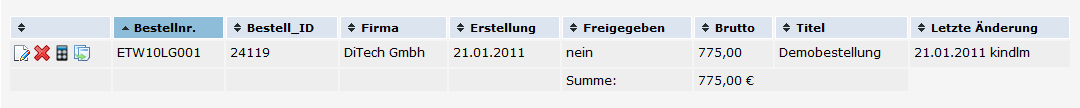
\includegraphics[width=1\textwidth]{gefundene_bestellungen.png}
	\caption{Suchergebnis der Bestellungen}
	\label{gefundene_bestellungen}
\end{figure}

Abbildung \ref{gefundene_bestellungen} zeigt eine Zeile einer Ergebnisliste nach einer Suchabfrage. Sie k�nnen die Liste durch klicken auf die Spalten�berschriften sortieren.
Folgende M�glichkeiten haben Sie durch klicken auf den entsprechenden Button:
\begin{itemize}
	\item 
\includegraphics[height=3mm]{edit}: �ffnet das Bestellformular der Bestellung damit �nderungen vorgenommen werden k�nnen.
	\item 
\includegraphics[height=3mm]{delete_x}: Bestellungen, zu denen noch keine Rechnung vorhanden ist, k�nnen hiermit gel�scht werden.
	\item 
\includegraphics[height=3mm]{calculator}: Anlegen einer neuen Rechnung zu dieser Bestellung.
	\item \includegraphics[height=3mm]{copy}: Es wird eine Kopie der Bestellung angelegt.
\end{itemize}


\section{Rechnung}
\label{rechnung}

\subsection{Neue Rechnung eingeben}

Rechnungen werden haupts�chlich vom Zentraleinkauf eingegeben.
Bei der Abrechnung des Kassabuchs und bei Dienstreiseabrechnungen (siehe dazu auch Kapitel \ref{dienstreiseabrechnung}) ist es erforderlich,
dass Sie selbst eine Rechnung anlegen.

Sie haben mehrere M�glichkeiten, eine Rechnung einzugeben.
Entweder Sie suchen nach einer Bestellung und klicken in der Auswahlliste auf das Symbol f�r \textit{Rechnung} (siehe dazu Kapitel \ref{suche_nach_bestellung})
oder Sie klicken im Benutzerbereich unter \textit{Rechnung} auf \textit{Neu}. \\
Im Hauptfenster k�nnen Sie nun aus einem Drop-Down Men� die gew�nschte Kostenstelle eingeben,
zu der Sie eine Rechnung eingeben m�chten.\\
W�hlen Sie sie aus und dr�cken Sie auf die Schaltfl�che \textit{Weiter}.

Abbildung \ref{rechnung_neu} zeigt das Formular zum Eingeben neuer Rechnungen.

Neu ist hier die Auswahlm�glichkeit des Rechnungstyps sowie das Bezeichnungsfeld bei den Betr�gen.
Au�erdem kann nun auch das Transferdatum der Rechnung erfasst werden.

\achtung{Vergessen Sie nicht, die MWSt anzugeben}

Zum genauen Ablauf bez�glich der Eingabe des Transferdatums und der genauen Rechnungsbetr�ge siehe Kapitel \ref{workflows}

\begin{figure}
	\centering
	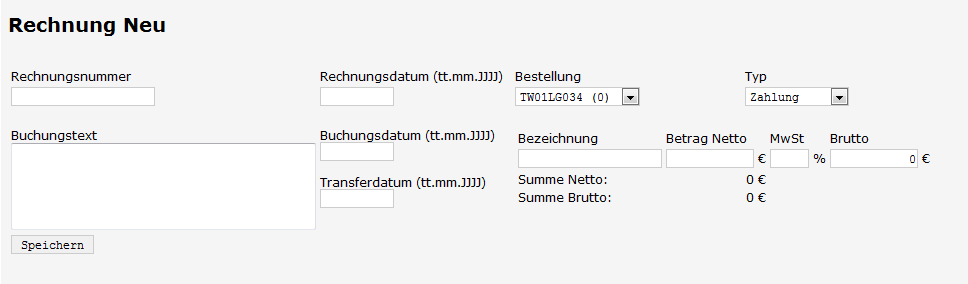
\includegraphics[width=1\textwidth]{rechnung_neu.png}
	\caption{Eingabeformular f�r neue Rechnungen}
	\label{rechnung_neu}
\end{figure}

\begin{description}
 \item [Rechnungsnummer:] Die Rechnungsnummer kann frei gew�hlt werden und aus Buchstaben und Zahlen bestehen.
 \item [Buchungstext:] Beliebiger Text.
 \item [Rechnungsdatum:] Datum der Rechnungslegung (auf der Rechnung).
 \item [Buchungsdatum:] Datum, an dem die Buchung vorgenommen wird (Standardeinstellung ist das heutige Datum).
 \item [Transferdatum:] Das Datum, an dem der Rechnungsbetrag tats�chlich �berwiesen wurde.
 \item [Bestellung:] W�hlen Sie hier die gew�nschte Bestellnummer aus, zu der die Rechnung angelegt werden soll.
 In der Auswahlliste k�nnen Sie erkennen, ob bereits eine Rechnung zu der Bestellnummer angelegt wurde.
 Die Zahl in der Klammer rechts neben der Bestellnummer gibt die Anzahl der vorhandenen Rechnungen an.
 Au�erdem werden Bestellungen ohne Rechnung gr�n hervorgehoben.
 \item [Typ:] Zahlungstyp. Zur Auwahl stehen:
 		\begin{itemize}
 		\item Zahlung
 	  \item Gutschrift
 	  \item Honorarnote
 		\end{itemize}
 		F�r eine genauere Beschreibung zur Verwendung der Zahlungstypen siehe Kapitel \ref{workflows}.
 	\item [Bezeichnung:] Eventuelle Beschreibung des Betrags. Nach Eingabe eines Betrags, wird automatisch eine neue Zeile hinzugef�gt.
 	\item [Betrag Netto:] Nettobetrag der Rechnung. Der Bruttobetrag wird automatisch nach Eingabe der Mehrwertsteuer berechnet.
	\item [MwSt:] Mehrwertsteuer auf dem Betrag.
	\item [Brutto:] Bruttobetrag der Rechnung. Der Nettobetrag wird automatisch nach Eingabe der MwSt angepasst.
\end{description}

\subsection{Suchen nach einer Rechnung}

Klicken Sie im Hauptmen� unter dem Punkt \textit{Rechnung} auf \textit{Suchen}. Hier k�nnen Sie nach vorhandenen Rechnungen suchen.

Abbildung \ref{rechnung_suchen} zeigt die Suchmaske, in der Sie folgende (optionale) Eingabem�glichkeiten haben:

\begin{figure}
	\centering
	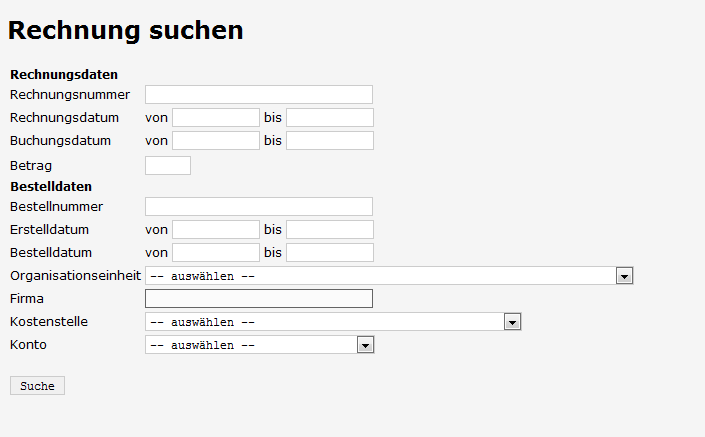
\includegraphics[width=1\textwidth]{rechnung_suchen.png}
	\caption{Suchmaske f�r Rechnungen}
	\label{rechnung_suchen}
\end{figure}

\begin{description}
	\item [Rechnungsnummer:] Sucht nach der kompletten Rechnungsnummer oder Teilen davon.
	\item [Rechnungsdatum/Buchungsdatum:] Wenn Sie in das Feld klicken, erscheint ein Kalender, aus dem Sie das gew�nschte Beginn- und Enddatum w�hlen k�nnen.
	Sie k�nnen das Datum auch direkt in der Form TT.MM.JJJJ eingeben.
	\item [Betrag:] Sucht nach einem bestimmten Netto- oder Brutto-Gesamtbetrag einer Rechnung.
\end{description}
Au�erdem k�nnen Sie die Suche mit Kriterien zu einer Bestellung verkn�pfen:
\begin{description}
	\item [Bestellnummer:] Sucht nach der kompletten Bestellnummer.
	\item [Erstelldatum/Bestelldatum:] Wenn Sie in das Feld klicken, erscheint ein Kalender, aus dem Sie das gew�nschte Beginn- und Enddatum w�hlen k�nnen.
	Sie k�nnen das Datum auch direkt in der Form TT.MM.JJJJ eingeben.
	\item [Organisationseinheit:] W�hlen Sie eine OE aus der Drop-Down Liste. Durchgestrichene OEs sind inaktiv.
	\item [Firma:] Auswahl der Firma, bei der bestellt wurde. Die Auswahlliste der Firma wird nach Eingabe von mind. zwei Zeichen gefiltert. Unter der Firmenbezeichnung wird die ID der Firma in der Datenbank angezeigt. Im Drop-Down Feld daneben werden die - zur OE zugeordneten - Firmen angezeigt, sofern welche vorhanden sind.
	\item [Kostenstelle:] W�hlen Sie hier die gew�nschte Kostenstelle aus.
	\item [Konto:] W�hlen Sie hier das gew�nschte Verrechnungskonto aus.
	\end{description}

\section{Firma}
\label{firma}

In der Firmenverwaltung k�nnen Sie neue Firmen anlegen und bestehende Eintr�ge suchen und bearbeiten.

Bitte �berpr�fen Sie vor dem Anlegen einer neuen Firma, ob diese nicht bereits im System existiert.
H�ufig werden Firmen mehrfach angelegt, was zu einem unn�tigen Datenberg f�hrt und letzlich auch Ihnen das Auffinden erschwert.

\subsection{Neue Firma anlegen}

Klicken Sie im Hauptmen� unter dem Punkt \textit{Firma} auf \textit{Neu} um eine neue Firma anzulegen.
Im erscheinenden Formular k�nnen Sie die Firmenbezeichnung, Adresse sowie Kontaktdaten eingeben.
F�llen Sie das Formular bitte so vollst�ndig wie m�glich aus.

\begin{figure}
	\centering
	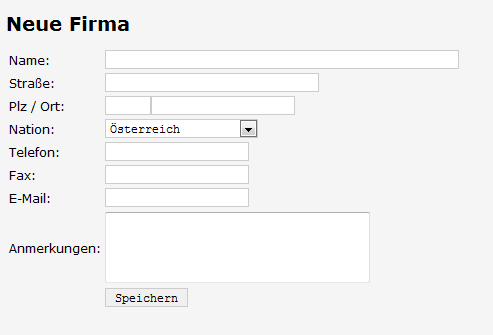
\includegraphics[width=0.5\textwidth]{firma_neu.png}
	\caption{Eingabeformular f�r einen neuen Firmenkontakt}
	\label{firma_neu}
\end{figure}

\subsection{Firma suchen}

Die Firmensuche sucht nach �bereinstimmungen innerhalb des Firmennamens, der Adresse und der ID im System.
Um eine �bersichtliche Ergebnisliste zu erhalten, sollten Sie mindestens 3 Zeichen bei der Suche eingeben.
\setlength{\baselineskip}{0.5cm}
\chapter{Administration}

Der Bereich der Administration ist nur bei entsprechender Berechtigung sichtbar.
Hier k�nnen Sie Konten und Kostenstellen anlegen und bearbeiten.

\section{Konto}
\label{admin_konto}

Durch einen Klick auf \textit{Konto} gelangen Sie zu einer �bersicht �ber alle derzeit angelegten Konten.
Mithilfe der Sybmole in der ersten Spalte k�nnen Sie einzelne Konten bearbeiten oder l�schen.

\subsection{Neu}
Der Men�punkt \textit{Neu} �ffnet ein Formular, in dem Sie ein neues Konto anlegen k�nnen.

\subsection{Zusammenlegen}
Die Praxis zeigt, dass gelegentlich �berfl�ssige Konten angelegt werden (zum Teil unbeabsichtigt), die in dieser Oberfl�che zusammengelegt werden k�nnen.
Die Oberfl�che zeigt zwei idente Listen, aus denen jeweils das �berfl�ssige (wird gel�scht) und das korrekte (bleibt erhalten) Konto durch klicken auf den Radio-Button am Ende jeder Zeile markiert wird. Anschlie�end werden die beiden Konten durch bet�tigen des Buttons \textit{->} vereint.

\section{Kostenstelle}
\label{admin_kostenstelle}
Durch einen Klick auf \textit{Kostenstelle} gelangen Sie zu einer �bersicht �ber alle derzeit angelegten Kostenstellen.
Mithilfe der Sybmole in der ersten Spalte k�nnen Sie einzelne Konten bearbeiten oder l�schen.
Au�erdem k�nnen Sie hier jeder Kostenstelle die entsprechenden Konten zuweisen.

\subsection{Neu}
Der Men�punkt \textit{Neu} �ffnet ein Formular, in dem Sie eine neue Kostenstelle anlegen k�nnen.

\subsection{Zusammenlegen}
Die Praxis zeigt, dass gelegentlich �berfl�ssige Kostenstellen angelegt werden, die in dieser Oberfl�che zusammengelegt werden k�nnen.
Sie sehen hier zwei idente Listen, aus denen jeweils die �berfl�ssige (wird gel�scht) und die korrekte (bleibt erhalten) Kostenstelle durch klicken auf den jeweiligen Radio-Button markiert wird. Anschlie�end werden die beiden markierten Kostenstellen durch bet�tigen des Buttons \textit{->} vereint.

\subsection{Budgeteingabe}
Hier k�nnen Sie f�r jede Kostenstelle das verf�gbare Budget im jeweiligen Gesch�ftsjahr eintragen.
W�hlen Sie aus dem Drop-Down Men� das gew�nschte Gesch�ftsjahr und klicken Sie auf \textit{Anzeigen}
Danach k�nnen Sie bei den gew�nschten Kostenstellen das Budget eingeben. Speichern Sie Ihre Eingaben mit dem Button am Ende der Liste.


\setlength{\baselineskip}{0.5cm}
\chapter{Berichte}

Sie k�nnen sich in diesem Abschnitt verschiedene Statistiken generieren lassen,
um sich einen �berblick �ber die angefallenen Kosten und Ausgaben zu verschaffen.

\section{Kostenstelle}
\label{bericht_kostenstelle}

\begin{figure}
	\centering
	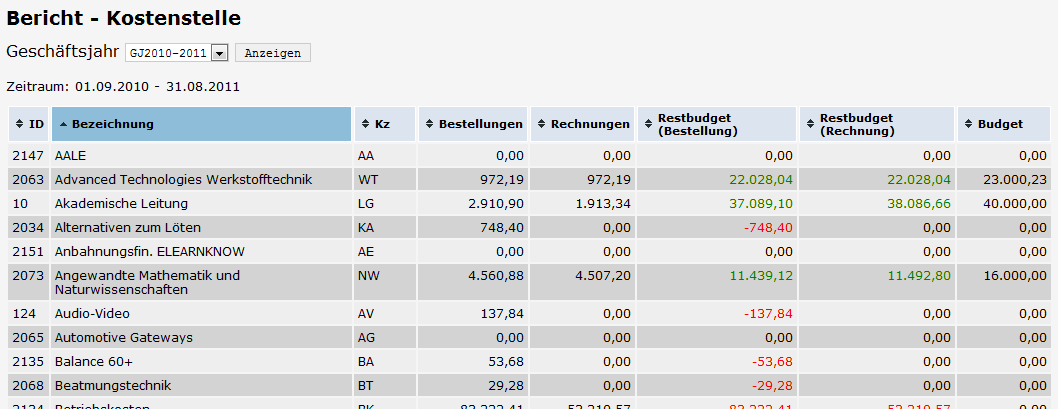
\includegraphics[width=1\textwidth]{bericht_kostenstelle.png}
	\caption{�bersicht �ber die Kostenstellen}
	\label{bericht_kostenstelle_screenshot}
\end{figure}

Nach der Auswahl des gew�nschten Gesch�ftsjahres aus dem Drop-Down Men�, wird Ihnen eine Auswertung �ber alle vorhandenen Kostenstellen erstellt.
Den verschiedenen Spalten (welche Sie durch einen Klick auf die �berschrift auch sortieren k�nnen) k�nnen Sie zB. die Bestellsumme oder das Restbudget entnehmen.

\section{Tags}
\label{bericht_tags}

Mithilfe der Checkboxen k�nnen Sie die gew�nschten Kostenstellen markieren, welche bei der Statistik ber�cksichtigt werden sollen.
W�hlen Sie anschlie�end das gew�nschte Gesch�ftsjahr aus dem Drop-Down Men� und klicken Sie auf \textit{Anzeigen}.

\begin{figure}
	\centering
	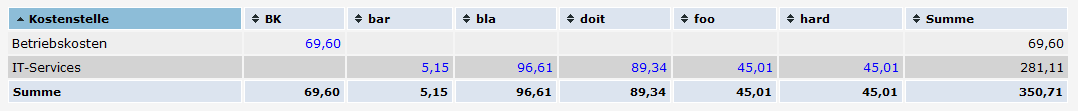
\includegraphics[width=1\textwidth]{bericht_tags.png}
	\caption{Auswertung der verwendeten Tags}
	\label{bericht_tags_screenshot}
\end{figure}

Abbildung \ref{bericht_tags_screenshot} zeigt ein Beispiel einer solchen Auswertung.
In den einzelnen Spalten sehen Sie alle, in der jeweiligen Kostenstelle verwendeten, Tags.
Der Summenzeile k�nnen Sie dann mit einem Blick entnehmen, wieviele Ausgaben in Bestellungen mit dem entsprechenden Tag get�tigt worden sind.

\info{Wenn Sie bei einer Bestellung oder Bestellposition mehrere Tags definiert haben, werden diese auch bei der Auswertung entsprechend mehrmals ber�cksichtigt und zur Gesamtsumme addiert. Zus�tzliche Tags verf�lschen also die Gesamtsumme.}

\section{Aufteilung}
\label{bericht_aufteilung}

Hier k�nnen Sie, einstellbar f�r das gew�nschte Gesch�ftsjahr, die Bruttokosten, aufgeteilt auf die einzelnen Organisationseinheiten, einsehen.
W�hlen Sie aus dem Drop-Down das gew�nschte Studiensemester und klicken Sie auf \textit{Anzeigen}, um das jeweilige Gesch�ftsjahr einsehen zu k�nnen.




\setlength{\baselineskip}{0.5cm}
\chapter{Besonderheiten im Bestellablauf}
\label{workflows}

\section{Zahlung per Nachnahme}
Der Begriff Nachnahme bedeutet, dass die Ware direkt beim Lieferanten bei der �bergabe der Ware bezahlt werden muss.
Diese Zahlungsform wird NICHT automatisch von allen Firmen angeboten.
Wenn Sie diese Form der Zahlung in Anspruch nehmen, haben Sie daf�r zu sorgen, dass der genaue Betrag \textbf{im Vorhinein} beim Empfang bzw. bei der Warenannahme hinterlegt ist.

\section{Dienstreiseabrechnung}
\label{dienstreiseabrechnung}
Die ben�tigten Formulare f�r die Abwicklung einer Dienstreise, finden Sie auf der CIS-Seite.

Stellen Sie zuerst einen Reiseantrag, den Sie von Ihrem/Ihrer Vorgesetzten abzeichnen lassen.
Nach Ihrer R�ckkehr, f�llen Sie die Dienstreiseabrechnung aus und lassen diese ebenfalls von Ihrem/Ihrer Vorgesetzten abzeichnen.
Erst danach legen Sie eine \textbf{Bestellung} und eine zugeh�rige \textbf{Rechnung} �ber den Gesamtbetrag im WaWi an.
Es ist nicht notwendig, alle Positionen einzeln bei der Bestellung und der Rechnung aufzuschl�sseln.

Die Dienstreiseabrechnung lassen Sie dann zusammen mit den Originalbelegen der Gesch�ftsf�hrung zukommen. Sie k�nnen die Abrechnung auch im Zentraleinkauf abgeben, welcher diese dann an die Gesch�ftsf�hrung weiterleitet.

Die Gesch�ftsf�hrung korrigiert dann ggf. die Betr�ge der Rechnung.

Damit sind von Ihrer Seite alle notwendigen Schritte durchgef�hrt.

\section{Honorarnote \normalsize{(ohne Lehrauftr�ge im FAS)}}
F�r Lehrauftr�ge, die ohnehin �ber das FAS abgerechnet werden, brauchen keine Honorarnoten gelegt zu werden.
Ein Formular f�r das Legen einer Honorarnote finden Sie ebenfalls auf der CIS-Seite.

F�llen Sie erst dieses Formular aus, lassen Sie es von Ihrem/Ihrer Vorgesetzten abzeichnen und legen Sie danach eine \textbf{Bestellung} und eine zugeh�rige \textbf{Rechnung} im WaWi �ber den Gesamtbetrag an.

Es ist nicht notwendig, alle Positionen einzeln bei der Bestellung und der Rechnung aufzuschl�sseln.

Die Honorarnote lassen Sie dann der Gesch�ftsf�hrung zukommen. Sie k�nnen die Honorarnote auch im Zentraleinkauf abgeben, welcher diese dann an die Gesch�ftsf�hrung weiterleitet.

Die Gesch�ftsf�hrung korrigiert dann ggf. die Betr�ge der Honorarnote.

Damit sind von Ihrer Seite alle notwendigen Schritte durchgef�hrt.

\section{Gutschrift}
Die Eingabe von Gutschriften ins WaWi wird vom Zentraleinkauf durchgef�hrt.

\section{Transferdatum und exakte Rechnungsbetr�ge}
Die exakten Rechnungsbetr�ge und das Datum der �berweisung liegen meist nur bei der Gesch�ftsf�hrung auf.
Um die Rechnungen richtig und vollst�ndig eingeben zu k�nnen, wird folgender Ablauf eingehalten:

\begin{itemize}
\item Einmal w�chentlich kommen die Rechnungsdaten der bezahlten Rechnungen von der Gesch�ftsf�hrung zum Zentraleinkauf.
\item Enthalten ist die Bestellnummer, der exakte Gesamtbetrag und das Transferdatum (Datum der tats�chlichen �berweisung).
\item Der Zentraleinkauf pflegt bis zur n�chsten Woche die Daten ins WaWi ein. Bestellungen werden nicht mehr korrigiert, nur mehr die Rechnungen.
\end{itemize}

Durch diese Vorgangsweise sollte im WaWi das exakte Restbudget ersichtlich sein und die Bestellungen k�nnen auch f�r die Budgetplanung genutzt werden. 

\section{Rechnung VOR Bestellung}
In der Praxis kommt es vor, dass Rechnungen ohne dazugeh�riger Bestellung vorliegen.
In diesem Fall ist es notwendig, zuvor eine Bestellung anzulegen, zu welcher die Rechnung zugeordnet werden kann.

\section{�ndern der Kostenstelle einer Rechnung}
H�ufig wird eine Bestellung zu Beginn auf die falsche Kostenstelle gebucht. Die Bestellnummer enth�lt dann das K�rzel der falschen Kostenstelle.
Solange die Bestellung noch nicht abgeschickt wurde, kann die Bestellnummer von einem Administrator ge�ndert werden.

Nach dem Abschicken, kann zwar die zugeh�rige Kostenstelle ge�ndert werden, jedoch muss die Bestellnummer unver�ndert bleiben.
H�ufig f�hrt dies zu Verwirrungen, wenn bei den eigenen Kostenstellen fremde K�rzel auftauchen.

\textbf{Die Bestellnummer hat also nicht immer einen Bezug zur Kostenstelle.}

\section{Innovationsscheck}
Gutschriften aus Innovationsschecks werden ausnahmslos von der Gesch�ftsleitung angelegt.
F�r jede Kostenstelle, die eine Gutschrift erh�lt, wird (\textbf{unabh�ngig von der Kostenstelle des Innovationsschecks}) eine Sammelbestellung von der GL erstellt.
Jede Gutschrift wird dort als eigene Bestellposition mit \textbf{negativem Betrag} ausgewiesen.

Pro Kostenstelle und Gesch�ftsjahr gibt es demnach eine eigene Bestellung, mit den entsprechenden Gutschriften.

Um jederzeit Eintragungen vornehmen zu k�nnen, darf die Bestellung nicht freigegeben werden.
Die gleiche Vorgehensweise gilt auch f�r die dazugeh�rigen Rechnungen.

\begin{figure}
	\centering
	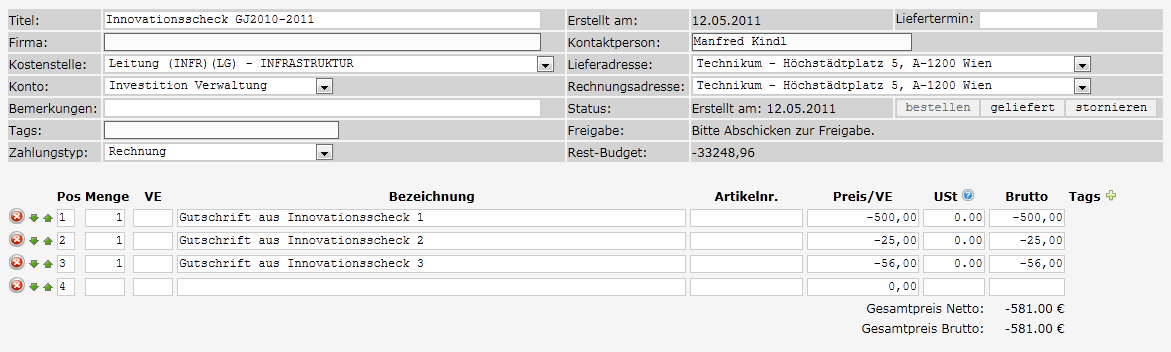
\includegraphics[width=1\textwidth]{innovationsscheck.png}
	\caption{In dieser Abbildung wurde zB. f�r die Kostenstelle "`Infrastruktur"' eine Sammelbestellung angelegt. Darin enthalten sind Gutschriften aus 3 verschiedenen Innovationsschecks.
	Der Kostenstelle "`Infrastruktur"' wird somit der Gesamtbetrag aus allen 3 Innovationsschecks gutgeschrieben.}
	\label{innovationsscheck}
\end{figure}

%% Kapitel Ende   %%%%%%%%%%%%%%%%%%%%%%%%%%%%%%%%%%%%%%%%%%%%%%%%%
\appendix							% Beginn des Anhangs
%%\chapter{Schluss}
%\listoftables					% Tabellenverzeichnis
%\listoffigures				% Abbildungsverzeichnis
\end{document}
